% autor: Paweł Mleczko <pml@amu.edu.pl> Pliki praca-dyplomowa.cls oraz
% praca.tex są objęte licencją Creative Commons BY-NC-SA szczegóły
% http://creativecommons.org/licenses/by-nc-sa/3.0/pl/legalcode

% Zastrzeżenie:
% Pliki praca-dyplomowa.cls zawiera zmiany w stosunku do oryginału, plik 00_main.tex bazuje na pliku praca.tex i również zawiera zmiany do niego.

\documentclass{praca-dyplomowa}
%% kodowanie, ustawienia językowe
\usepackage[utf8]{inputenc}
\RequirePackage[bitstream-charter]{mathdesign}
% \RequirePackage[T1]{polski}
\usepackage[
backend=biber,
style=apa,
citestyle=authoryear
]{biblatex}
\usepackage[colorlinks]{hyperref}
\usepackage{amsmath}
\usepackage{float}
\usepackage{graphics}
\usepackage{svg}


%
%% meta dane
%% tytuł pracy
\title{On Hadamard matrices and probabilistic data structures in neural networks}  
% %% tytuł w języku angielskim
% \entitle{On Hadamard Matrix and probabilistic data structures in neural networks}         
%% imię i~nazwisko autora pracy
\author{Ksawery Smoczyński}          
%% numer albumu
\album{2137}                        
%% nazwisko promotora
\promotor{dr Dorota Blinkiewicz}     
%% rok obrony pracy
\year{2024}                     
%% rodzaj pracy
\type{licencjacka}              
%% kierunek studiów
\course{matematyka}             
 %% specjalność studiów (proszę skonsultować w dziekanacie)
\speciality{finansowa i aktuarialna}     
%% potrzebne do oświadczenia
\date{20.06.2016}
\gender{\male}                  %% należy wybrać \male lub \female 
\Sfirst{TAK/NIE}                %% proszę wpisać TAK lub NIE (zgoda na udostępnienie pracy w~czytelni)  
\Ssecond{TAK/NIE}               %% proszę wpisać TAK lub NIE (zgoda na ochronę praw autorskich)
%
\italicsStyle
\newtheorem{theorem}{Theorem}
\newtheorem{lemma}{Lemma}
\newtheorem{wniosek}{Wniosek}
%
\plainStyle
\newtheorem{definition}{Definition}
\newtheorem{remark}{Remark}
\newtheorem{example}{Example}

% Bibliografia
\addbibresource{bibliography/01.bib}
\addbibresource{bibliography/05.bib}

\begin{document}
%% strona tytułowa pracy
\Titlepage      
 %% oświadczenie 
\Statement      
%% spis treści
\tableofcontents 

% Orginalny template można znaleźć tu:
% https://mleczko.faculty.wmi.amu.edu.pl/git/praca-dyplomowa.git

% Praca
\begin{streszczenie}
Streszczenie po polsku będzie tu!
\end{streszczenie}
\begin{abstract}
Here will be abstract
\end{abstract}

\begin{acknowlegements}
Tralalaal
\end{acknowlegements}
\section*{DRAFT: Introduction and motivation}
\subsubsection{Objectives and contributions}
What are the aims of this thesis:
\begin{itemize}
    \item Reduction of number of parameters?
    \item Verify if sparse redundant inputs to NNs could be effectively aggregated and processed without imposing any or little implicit bias by employing Hadamard matrix as a "mixing" operator.
\end{itemize}
\section{DRAFT: Literature review}
\subsection{Parameter efficiency in neural networks}
\begin{itemize}
    \item \href{https://arxiv.org/abs/1810.02309}{Compressed transforms}
\end{itemize}
\subsubsection{LoRA}
\begin{itemize}
    \item \href{https://arxiv.org/pdf/2402.09353.pdf}{DoRA}
\end{itemize}
\subsubsection{Other}

\subsection{Probabilistic data structures}
\subsubsection{Count-min sketch and locality sensitive hashing}
\subsubsection{EMDE: Efficient Manifold Density Estimator}

\subsection{Hadamard Matrix}
Hadamard Matrices firstly constructed by \cite{05_sylvester_construction} and proved by \cite{05_hadamard_maximal_determinant} to attain the bound for maximum determinant of all matrices of such kind, sparked interest across scientific disciplines and since then were studied extensively starting from theoretical mathematics with applications in the signal processing, coding theory, experimental design et cetera. In following subsection definition and all relevant properties of Hadamard matrices, that further experiments will take use of, will be introduced, secondly it's derived algorithmic form - Walsh-Hadamard transform will be described as it's the exact form how the Hadamard matrix will be used in practice in the network architecture in subsequent chapter \ref{06:AutomorpherNetwork}, finally it's relation to maximum determinant problem, maximal set of pairwise independent variables and optimal coding theory will be brought up in order to sketch the intuition and heuristic why it might be a good tool for the problem this thesis is trying to solve.

% Introduction and motivation, heuristic and intuition behind use. 
% \href{https://chaos.if.uj.edu.pl/~karol/pdf/TZ06.pdf}{UJ ładny wstęp}
% \href{https://www.sciencedirect.com/science/article/pii/0097316576900625}{WAllis 1972}
% \cite{05_hedayat_wallis_hadamard_matrices}

\begin{definition}
\label{05:HM:definition}
\noindent We call square matrix $H_{n}$ of order $n$ Hadamard matrix if:
\begin{enumerate}
    \item it's a square matrix of order $n \in \{1, 2\} \; \bigcup \;\{\;4k \quad | \quad k \in \mathbb{N}\}$
    \item all of it's entries are either $+1$ or $-1$
    \item all of it's rows are pairwise orthogonal
\end{enumerate}    
\end{definition}

% $$\{n,m \in \mathbb{N}, H \in M\{n, m\}(K) \quad | \quad n = m \quad \land \quad K = \{-1, 1\} \quad \land \quad \forall_{1<i<n, 1<j<m} h_{i, j} \in K \}$$ 
\subsubsection{Properties}
Additionaly matrix defined above have following properties. Firstly, from the fact that $H_n$ has orthogonal rows and consists only of entries from ${{1, -1}}$, following equality can be obtained:
\begin{equation} 
\label{05:HM:eq01}
    HH^{T} = nI    
\end{equation}
As $n$ is a scalar equation \ref{05:HM:eq01} can be rewritten as 
\begin{equation}
    H(n^{-1}H^{T}) = I    
\end{equation}
Therefore matrix $H$ is invertible with it's inverse equal to $n^{-1}H^T$. While substituting $\bar{H}$ for $H^T$ and $\bar{H}^T$ for $H$ formula stays valid, therefore it also can be concluded that pairwise orthogonality property also applies to Hadamard matrix columns.
From that it can be stated that matrix is Hadamard if it's transposition is also a Hadamard matrix.

% TODO: PROPERTY that permutation of rows yields equivalent hadamard matrix. Also what happens when we'll multiply by -1.

\subsubsection{Construction}
\label{05:HM:Construction}

There are various ways to construct Hadamard matrix, which depending on application might be of greater relevance to the problem that others. In this work original construction proposed by \cite{05_sylvester_construction} will be provided in this section, as well as the construction related to the Hadamard-Walsh {\color{red} \textbf{CITE}} transform in the subsection \ref{05:sub_hadamard_walsh} which will be de facto method used further during implementation. Except for those two, amongst others that could be mentioned Payley introduced a method based on the prime powers {\color{red} \textbf{CITE}}, which was further generalized by Wiliamson {\color{red} \textbf{CITE}}. For a more extensive overview of the construction methods \cite{05_hedayat_wallis_hadamard_matrices} can be of interest for the reader.

Let $\bigotimes$ denote Kronecker product. For the matrix $A$ with $n$ rows and $m$ columns and $B$ with $j$ rows an $i$ columns, where $a_{nm}$ is a entry in the $A$ matrix and $b_{ji}$ is an entry in the $B$ matrix, it's defined as:
\begin{equation}
    A \bigotimes B = \begin{bmatrix}
                    a_{11}B  & a_{1,2}B & \cdots  & \cdots & a_{1m}B \\
                    a_{2,1}B & a_{2,2}B &         &        & \vdots \\
                    \vdots   &          & \ddots  &        & \vdots \\
                    \vdots   &          &         & \ddots & \cdots \\
                    a_{n,1}B & \cdots   & \cdots  & \cdots & a_{n,m}B 
\end{bmatrix}
\end{equation}

Citing the theorem \cite{05_hedayat_wallis_hadamard_matrices}, higher order Hadamard matrices can be easily constructed by repeatably applying Kronecker product to the already constructed ones.
\begin{theorem}
If $H_n$ is a Hadamard matrix of order n and $H_m$ is a Hadamard matrix of order $m$ then $H_n \bigotimes H_m = H_nm$  
\end{theorem}
Let's introduce example for this fact to become obvious. Following notation from \cite{05_hedayat_wallis_hadamard_matrices} $\{-, +\}$ entries in the matrix will correspond to $\{-1, 1\}$ values.
Given that $H_n$ is a Hadamard matrix of order $n$ and $\begin{bmatrix}
    H_n & H_n \\
    H_n & -H_n \\
\end{bmatrix}$ yields Hadamard matrix of order $2n$.
From this a sequence of matrices can be constructed such as:
\begin{align*}
H_1 &= \begin{bmatrix}+\end{bmatrix} \\
H_2 &= \begin{bmatrix}+ & + \\ + & -\end{bmatrix} \\
H_4 &= \begin{bmatrix}
        + & + & + & + \\ 
        + & - & + & - \\
        + & + & - & - \\
        + & - & - & + 
        \end{bmatrix} =  
        \begin{bmatrix}
            H_2 && H_2 \\
            H_2 && -H_2
        \end{bmatrix} = 
        H_2 \bigotimes H_2
\end{align*}
Constructing following matrices in the same manner as above for higher orders yields more general formula.
\begin{equation}
\label{05:HM:recursive_definition}
    H_2 \bigotimes H_{2^{k-1}} = 
    \begin{bmatrix}
        H_{2^{k-1}} && H_{2^{k-1}} \\
        H_{2^{k-1}} && -H_{2^{k-1}}
    \end{bmatrix} = 
    H_{2^k}
\end{equation}
In this way Hadamard matrices of an arbitrary order $2^{k}$ can be defined for every $k \in \mathbf{Z}_+$, hence, the lemma:
\begin{lemma}
    For each $k \in \mathbf{Z}_+$ exists a Hadamard matrix of order $2^k$ 
\end{lemma}

\subsubsection{Walsh-Hadamard transform}
\label{05:sub_hadamard_walsh}
\href{https://www.mathworks.com/help/signal/ug/walshhadamard-transform.html}{OPIS}
So far in this section introduced the definition and construction of Hadamard Matrices. In the following subsection it's application as a linear transform will be investigated via introduction of so called Hadamard-Walsh transform which found it's application amongst many in signal processing {\color{red} \textbf{CITE}}. The neural network architecture which will be introduced in the next chapter \ref{06:AutomorpherNetwork}, will be utilizing it for initial preprocessing of the input vectors. 
Let's introduce notion of sequency (a generalized frequency) defined as a half of the of the average number of signal crossing zero in a unit of time. 
Ordering rows of Hadamard matrix by the number of the sign changes results in obtaining the Walsh matrix.
Walsh-Hadamard transform is an example of generalized class of Fourier transform, as it decomposes vector into superposition of Walsh functions. Each of the Walsh functions corresponds to  aforementioned sequency. Looking at it from this lens multiplying vector of the i.i.d random variables with it, allows for the what will be onwards referred to as mixing - linear combination of those. Recovery of the original vector is performed by multiplication with it's inverse. Why it will be relevant will be introduced in the following section \ref{06:AutomorpherNetwork}.
Fast Walsh-Hadamard transform is based on the recursive definition \ref{05:HM:recursive_definition} with additional normalization factor (which may be grouped together due to the associative property of scalar matrix multiplication):
\begin{equation}
    H_n = \frac{1}{\sqrt{2}}\begin{bmatrix}
        H_{n-1} && H_{n-1} \\
        H_{n-1} && -H_{n-1}
    \end{bmatrix}
\end{equation}
As it is known from the previous section Hadamard matrix has orthogonal rows and columns, scaling it ensures that its determinant is also equal to 1, therefore it's a linear transform which also preserves volumes - this results in  orthogonal matrix.

Dividing both sides of the equation by $n$ \ref{05:HM:eq01} and applying associative property of scalar matrix multiplication yields scaled matrices which are equal to identity matrix. Given that fact it's obvious that one of the products is an inverse of the other. Also, from the properties of Hadamard matrix it's transpose was shown to be itself. 
\begin{align*}
    HH^{T} &= nI \\
    \frac{HH^{T}}{n} &= I \\
    \frac{H}{\sqrt{n}}\frac{H^{T}}{\sqrt{n}} &= I \\
    det(\frac{H}{\sqrt{n}}\frac{H^{T}}{\sqrt{n}}) &= det(I) = 1 \\
    det(\frac{H}{\sqrt{n}})det(\frac{H^{T}}{\sqrt{n}}) &= det(I) = 1
\end{align*}
Therefore it can be seen that scaled down version of matrix has a determinant equal to 1. 

The algorithm for the Fast Walsh-Hadamard proceeds in a simple divide-and-conquer scheme depicted on the figure, with computational complexity of $O(nlogn)$ compared to the naive $O(n^2)$ matrix multiplication.
\ref{05:fig:fast_WHT_figure}.
\begin{figure}[H]
\label{05:fig:fast_WHT_figure}
\centering
\includesvg[width=250pt]{figures/05_literature_review/fast_WHT.svg}
\caption{Fast Walsh-Hadamard transform for the input vector $\begin{bmatrix}
    1 & 0 & 1 & 0 & 0 & 1 & 1 & 0
\end{bmatrix}^T$ \newline Source: Wikipedia \cite{FastWalshTransform}}
\end{figure}



\subsubsection{Relation of Hadamard matrix to maximal determinant problem, maximal set of pairwise independent variables and optimal coding theory}
In this subsection interpretation and heuristic which was basis for usage of Hadamard matrix for solving this thesis objectives will be introduced by relating its properties to other problems. 
First one is the primary reason why Hadamard started investigating this type of matrices, they were primarily found to be a solution to the so called "Hadamard's maximal determinant problem". The question asked was what is the upper bound for the determinant of order $n$ matrix with $\{-1, 1\}$ entries \cite{05_hadamard_maximal_determinant}. For the arbitrary $n$ this problem remains unsolved, however bound obtained by Hadamard states that for above-mentioned matrices determinant can maximally attain $n^{n/2}$. Moreover he showed that matrices constructed via Sylvester method introduced in previous section \ref{05:HM:Construction} reach this bound. 
In the Hadamard-Walsh transform description from the previous section normalizing factor was mentioned, normalizing Hadamard matrix ensures that it's determinant is equal to 1, therefore the transform preserves volumes. This results in the orthogonal matrix, which can be seen as a stiff rotations, reflections or combination of those of vectors. Not reaching the bound would imply that some of the rows or columns aren't orthogonal, therefore even though with proper scaling property of volume preservation would be attained it no longer would be an orthogonal matrix. {\color{red} \textbf{MAKE THIS ARGUMENT STRONGER OR MORE ELABORATE}}.
\par Another relationship that can be established is the one between Hadamard Matrix and maximal set of pairwise independent variables. 
Following \cite{05_hedayat_wallis_hadamard_matrices} by $R$ denote set ${X_1, X_2, \dots, X_k}$ of $k$ pairwise independent random variables on the set of $n$ points. Relaxing bound known from mutual independence equal to $v \leq log_2n$ to pairwise independence yields bound equal to $v \leq n-1$.
 bring up a theorem established by \cite{05_lancaster_maximal_set_of_pairwise_independent_variables}. 
\begin{theorem}
    The existence of a maximal set of pairwise independent random variables on n points (such that each of its members assigns the measure $n^{-1}$ to each point) is equivalent to the existence of a Hadamard matrix of order n.
\end{theorem}

There is a proof of this fact provided in the article Hedayat and Wallis article, which relies on the orthogonality of the columns of the Hadamard matrix. Below a proof provided by author might be not as concise but maybe more elaborate and therefore simpler to understand. In the essence both proofs rely on the same properties. 

Let's call Hadamard matrix normalized if it's first row and column both contain only $1$ as entries. Semi-normalized Hadamard matrix will be defined as Hadamard matrix with only $1$ as entries either for it's first row or column. Matrix $\hat{H}$ is obtained by removing first column from the semi-normalized Hadamard matrix.

\begin{proof}
Niech dana będzie przestrzeń probabilistyczna $(\Omega, \mathcal{A}, P)$, gdzie definiujmy zdarzenie elementarne $\omega$ jako liczbę ze zbioru $\{1,2,3, \dots, 4m\} = \Omega$ moc tego zbioru jest równa $4m=n$, $\sigma$-algebra $\mathcal{A}$ utożsamiamy ze zbiorem potęgowym zbioru zdarzeń elementarnych $2^{\Omega}$, oraz miarę $P$ które przyporządkowuje każdemu ze zdarzeń elementarnych równe prawdopodobieństwo równe $n^{-1}$.

Aby pokazać wzajemną niezależność dowolnych dwóch zmiennych losowych musimy pokazać, że $\forall_{i,j in \{1,2,3, \dots, n-1\} \colon i!=j} P(X_i)P(X_j) = P(X_iX_j)$.

Zdefiniujmy zmienne losowe $X_i \colon \Omega \to \{1,-1\}$ dla $i \in \{1, 2, 3, \dots, n-1\}$, które przyporządkowują wartości danego zdarzenia elementarnego wartość spod odpowiadającego jej indeksu z i-tej kolumny macierzy $\hat{H}$. Innymi słowy $X_i(\omega) = \hat{H}_{i,\omega}$.

X, Y wektory długosci 4n o wyrazach +1i -1
Suma X = Suma Y = Suma X*Y = 0
Pokazac, ze liczba tych i, ze X[i] = Y[i] = 1 wynosi n.
Tak samo pokazac, ze liczba tych i, ze X[i] = 1 i Y[i] = -1 wynosi n itd. dla pozostałych kombinacji znaków 

To jest równowaine temu, ze X i Y są niezależnymi zmiennymi losowymi na zbiorze {1,2..., 4n} takim, ze prawd. dowolnego punktu jest Jednakowe i równe 1/4n

\end{proof}

\par The last relation that is worth pointing towards is that of coding theory and error correcting codes to Hadamard matrices. Briefly introducing coding theory, it lies on the intersection of a mathematics, information theory, computer science and even linguistics. It's purpose is to represent information via coding - translating it to the constant length sequences of code symbols which are called code words. This definition can cover variety of use cases but for purpose of this section, only binary codes will be considered as they reflect the nature of electronic circuits and can directly relate to the cardinality of Hadamard matrices entries. According to \cite{coding_types_irvine} four types of coding can be distinguished:
\begin{enumerate}
    \item Data compression (or source coding) 
    \item Error control (or channel coding)
    \item Cryptographic coding 
    \item Line coding
\end{enumerate}. The coding introduced will be an example of error control coding, the one which handles the problem of perturbation of signals in transmission via corrupting medium. 
Code in which all code words have equal length $n$ will be called block code. By alphabet set $A$ of $q$ symbols will be denoted. As here only binary codes will be considered $A = \{0, 1\}$. By stating that all of the code words have length $n$, one can form all $n$-tuples if $A^n$ is a vector space, given that $A$ is a finite field. Then a subset of $A^n$ vector space can be identified as a block code of $q$ symbols.
For the purpose of alleviating corruption of one code word into another, a notion of difference has to be formalized. For given tuples $\mathbf{x}, \mathbf{y} \in {A^n}$ such that $\mathbf{x} = (x_1, x_2, ..., x_n), \mathbf{y} = (y_1, y_2, ..., y_n)$ quantity $d$ defined as $|\{\forall_{i \in \{1,2, ..., n\}} (x_i,  y_i) : x_i \neq x_i)\}|$ defines Hamming distance. If minimum of Hamming distances between the codes is at least $d$, such code is refereed to as distance $d$ code. Two properties of a code are directly related to the value of $d$ - ability for code error detection and error correction. Error detection property allows for distinguishing between corrupted and correctly transmitted information, whereas error correction allows for recovering the original code word from the corrupted signal. Distance $d$ code  is $d-1$-error detecting and $\frac{d-1}{2}$-error correcting, both are upper bounds, hence large distance codes are desirable.
Code constructed out of $M$ code words each of length $n$ with (Hamming) distance $d$ and $q$ symbols, can be described with tuple $(n, M, d, q)$. For given $n$, $d$, $q$ code is optimal when $M$ reaches it's upper bound \cite{05_plotkin_binary_codes_with_specified_minimum_distance}.
As \cite{05_hedayat_wallis_hadamard_matrices} proved 
\begin{theorem}
    The existence of Hadamard matrix of order 4t implies the existence of following optimal codes $(4t, 8t, 2t, 2)$, $(4t-1, 4t, 2t, 2)$, $(4t, 8t, 2t-1, 2)$, $(4t-2, 2t, 2t, 2)$.
\end{theorem}
The proof and the exact construction of the codes are left to the interested reader in the \cite{05_hedayat_wallis_hadamard_matrices} article.

Concluding, Hadamard matrix can be perceived from several angles such as an linear transform maximizing determinant (volume scaling property) of the constrained family of linear transforms, orthogonal matrix, as a way to construct maximal set of pairwise independent variables and a way to construct codes maximally robust to corruption. 
Those properties led to the idea that it would be viable to encode sparse representations by projecting them via Hadamard matrix and as a result obtain representation which would combine information from independent dimensions, for further sequential  projections and aggregations within the neural network, without inducing unreasonable inductive bias in arbitrary grouping of the features which wouldn't be permutation invariant.





Pytania:
Czy wyskalowana macierz Hadamarda jest automorfizmem?

* Dokładne odnośniki -> do każdego twierdzenia, dowodu, własności
izometria
\section{DRAFT: Automorpher Network}
\label{06:AutomorpherNetwork}
This section will describe in detail the architecture of neural network and how it incorporated methods and entities described in section literature review in order to alleviate problems mentioned in introduction section.
\section{DRAFT: Results of experiments}
Results here
\section{DRAFT: Summary and conclusions}
Summary here
% Do usunięcia w ostatecznej pracy
\section{NOTATKI}
\subsection{linki}
\begin{itemize}
    \item \href{https://uam.sharepoint.com/sites/4204000000/SitePages/Dyplomowanie-na-kierunku-Matematyka.aspx}{Wymagania co do pracy}
    \item \href{https://truben.no/latex/bibtex/}{GENEROWANIE BIBTEXów}
\end{itemize}
\section{Kilka słów o~zasadach typografii}

\noindent Proszę o~używanie następujących zasad:
{\raggedright
\begin{itemize}
\item nie zostawiać na końcu wiersza tzw. ,,wiszących spójników''
  (np. w, z...)
\item pisać \verb|\dywiz| w~miejsce -, czyli np.
  \verb|biało\dywiz czerwony| zamiast \verb|biało-czerwony|, ale
  \verb|$n$-wymiarowy|, a~nie \verb|$n$\dywiz wymiarowy|
\item pisać \verb|\polishendash| w~miejsce --, czyli
  np. \verb|twierdzenie Bolzano\polishendash Weierstrassa| a~nie
  \verb|twierdzenie Bolzano--Weierstrassa|
\item pisać półpauzę \verb|\ppauza|, czyli na przykład
  \verb|jak wspomnieliśmy\ppauza dowód jest poprawny|
\item pierwszy wiersz akapitu następujący po rozdziale lub punkcie bez
  wcięcia akapitowego (czyli \verb|\noindent|)
\end{itemize}\par}


\section{Zasada maksimum i~jej zastosowanie do badania szeregów
  potęgowych}

\noindent Celem tego rozdziału jest prezentacja zasady maksimum oraz
zastosowanie jej do badania szeregów potęgowych.

\subsection{Zasada maksimum}

\noindent Dowód poniższego twierdzenia można znaleźć na przykład
w~książce \cite{complex}.
\begin{theorem}[Zasada maksimum]\label{tw-1}
  Niech $\mathbb{D}$ będzie obszarem na płaszczyznie zespolonej.
  Jeśli $f\in H(\mathbb{D})$ oraz istnieje taki punkt
  $z_0\in\mathbb{D}$, że
  \[
  \sup \bigl\{|f(z)| : z\in\mathbb{D}\bigr\} =|f(z_0)|,
  \]
  to funkcja $f$ jest stała w~zbiorze $\mathbb{D}$.
\end{theorem}

\begin{proof}
\lipsum[1-4]
\end{proof}

\begin{definicja}
  Funcją całkowitą nazywamy finkcję mającą pochodną w~każdym punkcie
  płaszczyzny zespolonej.
\end{definicja}

\subsection{Suma szeregu geometrycznego}

\noindent Podstawową rolę w~dalszych rozważaniach odgrywać będzie
poniższe twierdzenie.

\begin{theorem}\label{tw-2}
  Jeśli $|x|<1$, to
  \begin{equation*}
    \sum_{n=0}^\infty x^n=\frac{1}{1-x}.
  \end{equation*}
\end{theorem}

\begin{proof}
  Ze wzoru na sumę skończonej ilości wyrazów ciągu geometrycznego
  wynika, że
  \begin{equation}\label{w-1}
    \sum_{k=0}^n x^k=\frac{1-x^{n+1}}{1-x}.
  \end{equation}
  Zauważmy teraz, że jeśli $|x|<1$, to granica wyrażenia stojącego po
  prawej stronie znaku równości we wzorze \eqref{w-1} istnieje oraz
  \[
  \lim_{n\to\infty} \sum_{k=0}^n x^k=\lim_{n\to\infty}
  \frac{1-x^{n+1}}{1-x} =\frac{1}{1-x}.
  \]
\end{proof}

Z~twierdzenia \ref{tw-2} otrzymać można (w~miejsce $x$ podstawiając
$-x$) poniższą równość.

\begin{wniosek}
Jeśli $|x|<1$, to 
\begin{equation}\label{w-2}
\sum_{n=0}^\infty (-1)^n x^n=\frac{1}{1+x}.
\end{equation}
\end{wniosek}

\lipsum[1-5]

\begin{uwaga}
  Podstawmy w~równościach \ref{w-1} oraz \ref{w-2} w~miejsce $x$
  wyrażenie $x^2$.  Poniżej prezentujemy otrzymane wykresy funkcji.

\begin{figure} 
  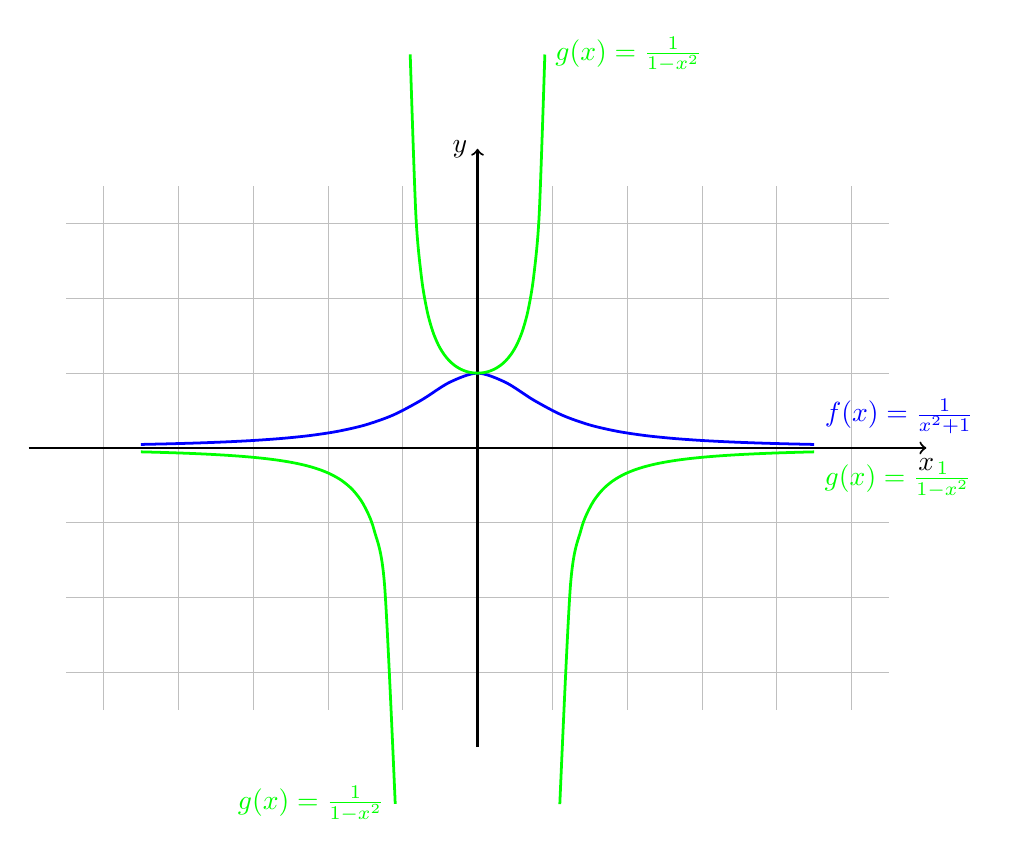
\begin{tikzpicture}[scale=.95]
\draw[step=1,lightgray,very thin] (-5.5,-3.5) grid (5.5,3.5);
\draw[line width=.75pt,->] (-6,0) -- (6,0) node[below] {$x$};
\draw[line width=.75pt,->] (0,-4) -- (0,4) node[left] {$y$};
%
\draw[line width=1pt,blue,variable=\x,smooth,domain=-4.5:4.5]
plot({\x},{1/(\x*\x+1)}) node[above right] {$f(x)=\frac{1}{x^2+1}$};
%
\draw[line width=1pt,green,variable=\x,smooth,domain=-4.5:-1.1]
plot({\x},{1/(1-\x*\x)}) node[left] {$g(x)=\frac{1}{1-x^2}$};
\draw[line width=1pt,green,variable=\x,smooth,domain=-.9:.9]
plot({\x},{1/(1-\x*\x)}) node[right] {$g(x)=\frac{1}{1-x^2}$};
\draw[line width=1pt,green,variable=\x,smooth,domain=1.1:4.5]
plot({\x},{1/(1-\x*\x)}) node[below right] {$g(x)=\frac{1}{1-x^2}$};
\end{tikzpicture}
\caption{Wykresy funkcji $f(x)=\frac{1}{x^2+1}$ (kolorem niebieskim)
  oraz $g(x)=\frac{1}{1-x^2}$ kolorem zielonym}
\end{figure}
\end{uwaga}

\section{Jak wykonywać rysunki w~programie \LaTeX?}

\noindent Celem tego rozdziału jest prezentacja sposobu przygotowania rysunków
z~wykorzystaniem pakietu \emph{tikz} w~programie \LaTeX.

\subsection{Proste rysunki}

\begin{center}
\begin{tikzpicture}
\draw (0,0) circle (3);
\draw (0,0) -- (3,3);
\draw (0,0) -- (3.5,0);
\draw[line width=.75pt] (1,0) arc (0:45:1);
\node[above] at (.5,0) {$\alpha$};
\end{tikzpicture}
\end{center}

\lipsum[1]

\subsection{Wykresy funkcji}

\noindent Można również rysować wykresy funkcji.

\noindent 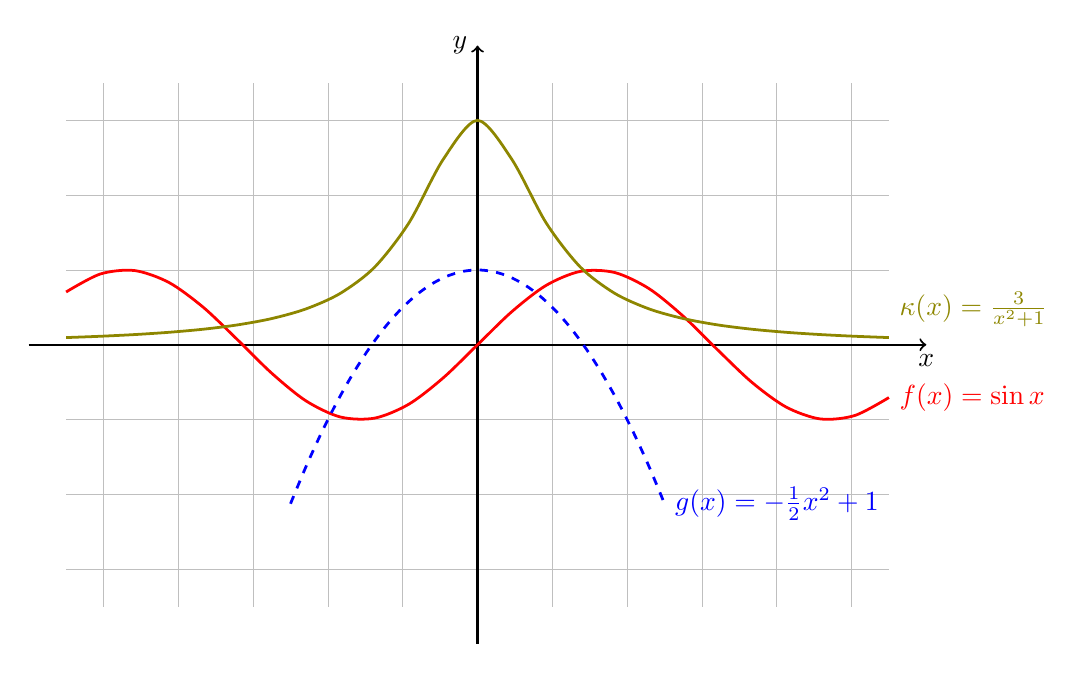
\begin{tikzpicture}[scale=.95]
\draw[step=1,lightgray,very thin] (-5.5,-3.5) grid (5.5,3.5);
\draw[line width=.75pt,->] (-6,0) -- (6,0) node[below] {$x$};
\draw[line width=.75pt,->] (0,-4) -- (0,4) node[left] {$y$};
\draw[line width=1pt,red,variable=\x,smooth,domain=-5.5:5.5]
plot({\x},{sin(\x r)}) node[right] {$f(x)=\sin x$};
\draw[line width=1pt,blue,dashed,variable=\x,smooth,domain=-2.5:2.5]
plot({\x},{-.5*\x*\x+1}) node[right] {$g(x)=-\frac{1}{2}x^2+1$};
\draw[line width=1pt,olive,variable=\x,smooth,domain=-5.5:5.5]
plot({\x},{3/(\x*\x+1)}) node[above right]
{$\kappa(x)=\frac{3}{x^2+1}$};
\end{tikzpicture}

\lipsum[1-6]

\printbibliography
\end{document}
